\documentclass[../tesis.tex]{subfiles}
\begin{document}

\chapter{Marco teórico}
\label{chapter:marco}

El presente capítulo expone los fundamentos teóricos y matemáticos que sustentan esta investigación.
Se abordan, en primer lugar, los conceptos clínicos de la densitometría ósea, el diagnóstico de la
osteoporosis y las modalidades multimodales que el equipo DXA genera más allá del T-score.
A continuación se detallan las arquitecturas algorítmicas de aprendizaje automático empleadas en
el análisis de clasificación transversal, las métricas de evaluación relevantes y los métodos de
interpretabilidad necesarios para la validación de modelos en el ámbito clínico.

% ─────────────────────────────────────────────────────────────────────────────
\section{Densitometría ósea, diagnóstico de la osteoporosis y modalidades DXA}
\label{sec:densitometria}
% ─────────────────────────────────────────────────────────────────────────────

La osteoporosis es una enfermedad esquelética sistémica de carácter metabólico, caracterizada por
la disminución de la masa ósea y el deterioro de la microarquitectura del tejido óseo, lo cual
conduce a un incremento sustancial en la fragilidad ósea y el riesgo de fracturas.
Clínicamente, el estándar de oro para su diagnóstico es la Absorciometría de Rayos X de Energía
Dual (DXA), una técnica radiológica bidimensional que cuantifica la Densidad Mineral Ósea (DMO).

De acuerdo con los criterios de la Organización Mundial de la Salud (OMS), el diagnóstico se
establece mediante el \textit{T-score}, una métrica que representa el número de desviaciones
estándar en las que la DMO del paciente se aleja de la media de una población adulta joven y sana
\cite{WHO1994}.
Un \textit{T-score} $\leq -2{,}5$ indica osteoporosis; valores entre $-2{,}5$ y $-1{,}0$ denotan
osteopenia; y valores $\geq -1{,}0$ se consideran normales.

A pesar de su adopción universal, el \textit{T-score} basado exclusivamente en la DMO presenta
limitaciones fundamentales al colapsar un sistema tridimensional complejo, capturado mediante una
proyección bidimensional, en un único escalar.
La resistencia mecánica del hueso depende no solo de la densidad, sino de la geometría, la
microarquitectura trabecular y la integridad cortical \parencite{AibarAlmazan2022}.
Para solventar esta brecha, los equipos DXA modernos ---como el GE Lunar Prodigy utilizado en
el CIMOHU--- proveen un conjunto de modalidades complementarias latentes que esta investigación
integra como \textit{features} predictivos.

\subsection{Análisis Estructural de Cadera (HSA)}
\label{subsec:hsa}

El \textit{Hip Structural Analysis} (HSA), desarrollado originalmente por \textcite{Beck1990},
deriva métricas de geometría ósea tridimensional directamente del escaneo DXA bidimensional
mediante análisis de la distribución de masa mineral a lo largo del cuello femoral.
Las variables clave incluyen la Longitud del Eje de la Cadera (HAL), el Área de Sección
Transversal (CSA), el Índice de Sección de Módulo Compuesto (CSMI) y el Ancho Cortical.
Estas métricas capturan la resiliencia estructural del hueso de forma independiente a la densidad
puntual, y representan 1.530 registros disponibles en la base de datos del CIMOHU.
Estudios longitudinales con DXA han demostrado que, tras una fractura de cadera, los pacientes
experimentan declives acelerados en el Módulo de Sección (SM) y el Área de Sección Transversal
(CSA), acompañados de aumentos compensatorios en el Diámetro Externo (OD) en las regiones del
cuello estrecho e intertrocantérea \cite{Rathbun2020_HSA}.
Estas trayectorias de degradación geométrica presentan variaciones significativas según el sexo
\cite{Rathbun2016_Sex} y se asocian a declives en la DMO entre 2{,}65 y 5 veces superiores (según el sitio anatómico) a los
observados en sujetos no fracturados de edad equivalente \cite{Rathbun2018_BMD}.
Estos hallazgos justifican la inclusión de los parámetros HSA como \textit{features} predictivos
independientes de la DMO en el \textit{pipeline} del presente proyecto.

\subsection{Evaluación de Fractura Vertebral (VFA)}
\label{subsec:vfa}

La \textit{Vertebral Fracture Assessment} (VFA) permite la detección semicuantitativa de
deformidades vertebrales mediante la medición de alturas anteriores, medias y posteriores de los
cuerpos vertebrales (T6--L4) a partir de una imagen de baja dosis de radiación obtenida en el
mismo examen DXA.
La clasificación semicuantitativa de \textcite{Genant1993} define tres grados de deformidad
---leve, moderada y severa--- según la reducción proporcional de altura vertebral respecto a la
vértebra de referencia.
El \textit{dataset} del CIMOHU contiene 2.499 registros de morfometría vertebral, que constituyen
una capa multimodal clave para el análisis de ablación previsto en el objetivo específico 3.

\subsection{Composición corporal regional}
\label{subsec:composicion}

El equipo DXA segmenta el cuerpo en regiones anatómicas ---cabeza, tronco, pelvis, extremidades
superiores e inferiores, zonas android y gynoid--- cuantificando independientemente la masa grasa,
la masa magra y la masa ósea por región.
Los 94.709 registros de composición corporal del CIMOHU son la segunda fuente de \textit{features}
más rica del \textit{dataset}, y su desglose regional permite modelar asimetrías y distribuciones
de grasa visceral que el Índice de Masa Corporal (IMC) global no captura.

La integración de la masa muscular magra es de particular relevancia debido al fenómeno fisiológico
de \textit{cross-talk} entre músculo y hueso, conocido clínicamente como \textbf{osteosarcopenia}:
la coexistencia de baja masa ósea (osteopenia u osteoporosis) y sarcopenia en el mismo individuo,
un síndrome revisado y sistematizado por \textcite{Kirk2020} que amplifica sinérgicamente el riesgo de caídas
y fracturas respecto al de cada condición por separado.

La base biológica de esta interacción es bidireccional \parencite{Kirk2020}: las miocinas secretadas
por el músculo esquelético ---miostatina, folistatina e irisina--- modulan directamente la
remodelación ósea (la miostatina induce osteoclastogénesis; la folistatina y la irisina inhiben
la resorción ósea), mientras que las osteocinas producidas por el hueso ---osteocalcina y
conexina~43--- regulan el anabolismo y catabolismo muscular en sentido inverso.
Adicionalmente, la acumulación de grasa intramuscular e intramedular propia del envejecimiento
secreta adipocinas que inducen apoptosis coordinada de miocitos y osteocitos.
Esta interacción tripartita músculo-hueso-grasa fundamenta la necesidad de capturar
simultáneamente variables de las tres categorías en cualquier modelo predictivo de riesgo
musculoesquelético.

Las consecuencias clínicas de la osteosarcopenia son cuantificables y superan las de sus componentes
aislados: en adultos mayores con ambas condiciones, el riesgo de caídas (OR: 2{,}83--3{,}63;
$p < 0{,}05$) y de fracturas (OR: 3{,}86--4{,}38; $p < 0{,}05$) es significativamente mayor
que en individuos sin osteosarcopenia \parencite{Kirk2020}.
Críticamente, a la fecha no existen herramientas de cribado ni modelos predictivos validados
específicamente para la detección de osteosarcopenia \parencite{Kirk2020}, lo que representa
una brecha directamente abordable por el enfoque multimodal propuesto en esta tesis.

El DXA posee la ventaja operativa de cuantificar simultáneamente la DMO y la masa magra
apendicular (ALM), de modo que ambas fuentes de información provienen del mismo equipo
y protocolo de adquisición.
\textcite{Kirk2020} demostraron que la sarcopenia es un predictor independiente de caída y
fractura, y que el deterioro muscular precede y agrava el óseo.
Esta asociación ha sido documentada en poblaciones de alto riesgo clínico: en adultos mayores
con infección por VIH estable, la masa muscular apendicular (ASMI) se correlacionó
significativamente con la DMO femoral y lumbar \parencite{Oursler2020}.
En el contexto local, \textcite{Barrientos2021} determinaron que la sarcopenia afecta a una
proporción significativa de adultos mayores costarricenses, validando la necesidad de incorporar
índices de composición corporal extraídos del DXA en los vectores predictivos.
Esta interconexión justifica incluir simultáneamente DMO, composición corporal, geometría
estructural y morfometría como \textit{features} predictivos, en línea con estudios que evidencian
que la fusión imagen+clínica mejora sobre modelos unimodales, aunque dichos estudios operan con
muestras limitadas y carecen de validación externa \parencite{Ong2023, Wu2025multimodal, Conforti2026}.
La Figura~\ref{fig:multimodal} ilustra conceptualmente cómo las cuatro modalidades del densitómetro
se integran, en principio, en un único vector de características que alimenta la escalera de
modelos de ML.

Sin embargo, en la base de datos del CIMOHU la cohorte de pacientes con T-score válido de columna
y/o cadera y la cohorte con escaneo de cuerpo completo (necesario para extraer composición
corporal) son \textbf{casi mutuamente excluyentes} ($n = 2.591$ y $n = 665$ respectivamente, con
solo 42 pacientes en común). Esta disyunción se explica porque el CIMOHU es utilizado con
frecuencia para análisis metabólicos generales ---evaluación nutricional y deportiva de
composición corporal en población relativamente joven--- y no exclusivamente como centro de
referencia para el diagnóstico de osteoporosis, lo cual explica también la juventud relativa de la
submuestra de cuerpo completo frente a la cohorte clásica de osteoporosis \parencite{Barrientos2021}.
Por esta razón, la contribución de la composición corporal al riesgo de osteoporosis se evalúa
mediante un modelo de ablación entrenado sobre la intersección real de ambas cohortes ($n = 42$
pacientes), de forma separada al modelo principal de clasificación transversal (Fase~2,
§~\ref{sec:fase2_multimodal}), en lugar de fusionarla directamente en un único vector de
\textit{features} para toda la cohorte.

\textbf{Indicio empírico propio, de carácter exploratorio: el tejido blando podría estar asociado a
la densidad ósea incluso en poblaciones jóvenes.} La evaluación preliminar de este modelo de
ablación sobre los datos del CIMOHU (Piloto B$'$, §~\ref{sec:resultados_pilotob}) es consistente con
la premisa teórica de esta sección, aunque con el carácter no concluyente propio de una muestra de
$n=42$. Mediante regresión con Validación Cruzada \textit{Leave-One-Out} sobre el T-score
continuo de los 42 pacientes de la intersección ---una sub-cohorte sistemáticamente más joven y
sana que la población clínica de referencia para osteoporosis, condición \textit{a priori} menos
favorable para detectar una asociación entre tejido blando y hueso---, las variables puramente
demográficas (edad, sexo, IMC) explican apenas el $12{,}4$\,\% de la varianza observada del T-score
($R^2 = 0{,}124$). Al incorporar las variables de composición corporal (masa grasa, masa magra y
porcentaje de grasa), el poder explicativo observado casi \textbf{se triplica} hasta un $38{,}1$\,\%
($R^2 = 0{,}381$), sin que esta diferencia se haya sometido a una prueba formal de significancia y
con el matiz de que el porcentaje de grasa es una función determinística de las otras dos
variables de composición incluidas en el mismo modelo, lo que introduce colinealidad
(§~\ref{sec:fase2_multimodal}). Este patrón preliminar es \textbf{compatible con} ---sin
constituir, por sí solo, prueba concluyente de--- la evidencia de la literatura internacional
\parencite{Edwards2015, Oursler2020} de que los tejidos blandos ---músculo y grasa--- se asocian
a la densidad ósea incluso en poblaciones jóvenes y relativamente sanas, lo que refuerza, junto con
esa literatura, la justificación científica para aislar y extraer estas variables del examen DXA
como \textit{features} predictivos independientes en la Fase~3, en lugar de descartarlas por la
limitada superposición muestral con la cohorte etiquetada principal.

\begin{figure}[h]
\centering
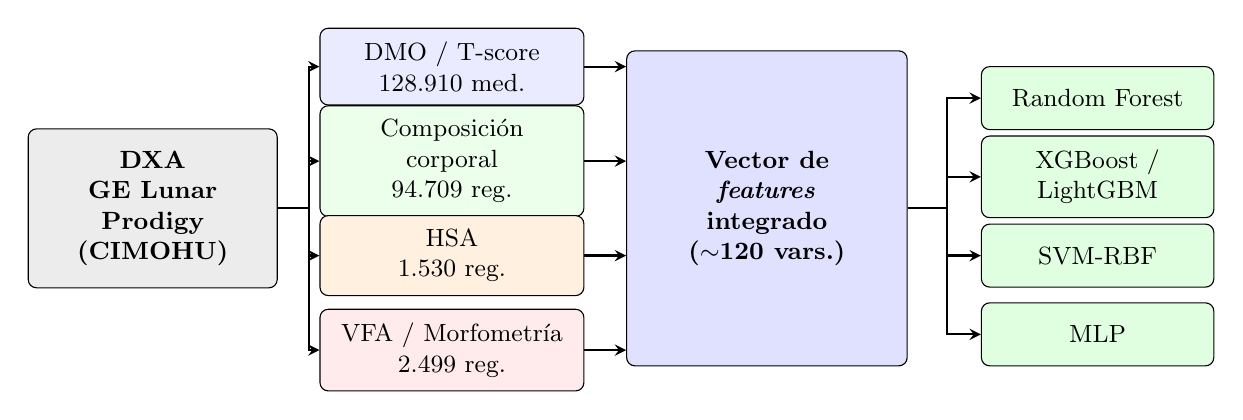
\begin{tikzpicture}[
  dxa/.style={draw, rounded corners=3pt, fill=gray!15, font=\small\bfseries,
              inner sep=8pt, text width=2.6cm, align=center, minimum height=1cm},
  mod/.style={draw, rounded corners=3pt, inner sep=5pt, text width=3.0cm,
              align=center, font=\small, minimum height=0.9cm},
  vec/.style={draw, rounded corners=3pt, fill=blue!12, inner sep=8pt,
              text width=3.0cm, align=center, font=\small\bfseries, minimum height=4.0cm},
  ml/.style={draw, rounded corners=3pt, fill=green!12, inner sep=5pt,
             text width=2.6cm, align=center, font=\small, minimum height=0.8cm},
  arrow/.style={->, thick, >=stealth}
]

% DXA source
\node[dxa] (dxa) at (0,0) {DXA \\ GE Lunar Prodigy \\ (CIMOHU)};

% 4 modalities
\node[mod, fill=blue!8]   (dmo) at (3.8, 1.8)  {DMO / T-score \\ 128.910 med.};
\node[mod, fill=green!8]  (cc)  at (3.8, 0.6)  {Composición \\ corporal \\ 94.709 reg.};
\node[mod, fill=orange!12](hsa) at (3.8, -0.6) {HSA \\ 1.530 reg.};
\node[mod, fill=red!8]    (vfa) at (3.8, -1.8) {VFA / Morfometría \\ 2.499 reg.};

% Feature vector
\node[vec] (fv) at (7.8, 0) {Vector de \\ \textit{features} \\ integrado \\ ($\sim$120 vars.)};

% ML models
\node[ml, fill=green!12] (rf)      at (12.0,  1.4) {Random Forest};
\node[ml, fill=green!12] (xgb)     at (12.0,  0.4) {XGBoost / LightGBM};
\node[ml, fill=green!12] (svm)     at (12.0, -0.6) {SVM-RBF};
\node[ml, fill=green!12] (mlp)     at (12.0, -1.6) {MLP};

% Arrows DXA → modalities
\draw[arrow] (dxa.east) -- ++(0.4,0) |- (dmo.west);
\draw[arrow] (dxa.east) -- ++(0.4,0) |- (cc.west);
\draw[arrow] (dxa.east) -- ++(0.4,0) |- (hsa.west);
\draw[arrow] (dxa.east) -- ++(0.4,0) |- (vfa.west);

% Arrows modalities → feature vector
\draw[arrow] (dmo.east) -- (fv.west |- dmo.east);
\draw[arrow] (cc.east)  -- (fv.west |- cc.east);
\draw[arrow] (hsa.east) -- (fv.west |- hsa.east);
\draw[arrow] (vfa.east) -- (fv.west |- vfa.east);

% Arrows feature vector → ML models
\draw[arrow] (fv.east) -- ++(0.5,0) |- (rf.west);
\draw[arrow] (fv.east) -- ++(0.5,0) |- (xgb.west);
\draw[arrow] (fv.east) -- ++(0.5,0) |- (svm.west);
\draw[arrow] (fv.east) -- ++(0.5,0) |- (mlp.west);

\end{tikzpicture}
\caption[Diagrama conceptual de la integración multimodal propuesta]{Diagrama conceptual de la integración multimodal propuesta. Las cuatro modalidades DXA generadas por el equipo GE Lunar Prodigy del CIMOHU se fusionan, en principio, en un vector de características unificado que alimenta la escalera de modelos de ML. En la práctica, dada la casi disyunción entre la cohorte con T-score y la cohorte con escaneo de cuerpo completo (§~\ref{subsec:composicion}), la composición corporal se evalúa mediante un modelo de ablación independiente sobre su propia submuestra (Fase~2, §~\ref{sec:fase2_multimodal}), mientras que el modelo principal integra DMO, demografía y HSA.}
\label{fig:multimodal}
\end{figure}

% ─────────────────────────────────────────────────────────────────────────────
\section{Aprendizaje automático para clasificación transversal}
\label{sec:ml_transversal}
% ─────────────────────────────────────────────────────────────────────────────

Para superar las limitaciones del enfoque umbral del diagnóstico clínico tradicional, se plantea
el uso de algoritmos de Aprendizaje Automático (ML) para clasificación supervisada.
Esta investigación emplea una escalera de complejidad que permite comparar el rendimiento
incremental de distintos enfoques bajo condiciones idénticas de datos y partición.

\subsection{Regresión logística}
\label{subsec:logistic}

La regresión logística es un modelo lineal interpretable que sirve como \textit{baseline} mínimo
junto al T-score umbral y al índice OST\@.
Establece el piso de rendimiento contra el cual se mide la ganancia de los modelos más complejos y
permite verificar que la señal del \textit{dataset} multimodal supera a la predicción univariada.
Este modelo se implementa como \textit{baseline} clínico en la Fase~3 de la metodología
(§~\ref{sec:fase3_transversal}).

\subsection{\textit{Random Forest}}
\label{subsec:rf}

\textit{Random Forest} es un método de ensamble basado en la construcción de múltiples árboles de
decisión durante el entrenamiento.
Utiliza técnicas de \textit{bagging} (muestreo con reemplazo) y selección aleatoria de
subconjuntos de características (\textit{random subspace}) en cada nodo, lo que lo hace altamente
robusto frente al ruido y a problemas de multicolinealidad.
Provee una estimación nativa de importancia de \textit{features} por reducción de impureza de
Gini, útil para el análisis de ablación multimodal previsto en el objetivo específico 3.
Este algoritmo se entrena en la Fase~3 (§~\ref{sec:fase3_transversal}); su importancia por
impureza complementa el análisis SHAP de la Fase~4 (§~\ref{sec:fase5_validacion}).

\subsection{XGBoost y LightGBM}
\label{subsec:xgboost}

XGBoost (\textit{eXtreme Gradient Boosting}) y LightGBM son algoritmos de ensamble basados en
árboles de decisión que emplean la técnica de \textit{gradient boosting}.
A diferencia de \textit{Random Forest}, construyen árboles de forma secuencial, donde cada nuevo
árbol se optimiza matemáticamente para corregir los residuos de los anteriores.
Incorporan regularización intrínseca (L1 y L2) para prevenir el sobreajuste y manejan datos
faltantes de forma nativa ---una ventaja crítica dada la naturaleza heterogénea del
\textit{dataset} del CIMOHU.

Estos algoritmos son los de mayor rendimiento en la literatura reciente de predicción de
osteoporosis: \textcite{Je2025} reportan un AUC de 0{,}84 con XGBoost, superando a ORAI (0{,}74)
y OST (0{,}71); \textcite{Jin2025} alcanzan AUC de 0{,}805--0{,}811 en validación transcultural;
\textcite{Carvalho2025} logran el techo actual del estado del arte con AUC 0{,}94 y exactitud
del 93\,\% mediante un ensamble de apilamiento que incluye XGBoost y LightGBM como estimadores
base ---aunque, como se discute en §~\ref{hipotesis}, sobre datos tabulares sin DXA y con una
variable objetivo no directamente comparable a la de este trabajo.
Ambos algoritmos se evalúan en la Fase~3 de la metodología (§~\ref{sec:fase3_transversal}),
donde forman la columna vertebral del ensamble de clasificación multimodal.

\subsection{\textit{Support Vector Machines}}
\label{subsec:svm}

Las \textit{Support Vector Machines} (SVM) proyectan los datos a un espacio de mayor dimensión
a través de una función \textit{kernel} ---como la Función de Base Radial (RBF)--- para encontrar
el hiperplano óptimo que maximiza el margen de separación entre clases.
Este método es altamente efectivo para capturar no linealidades complejas en datos biométricos y
fue el mejor predictor en el estudio seminal de \textcite{Yoo2013}, con AUC de 0{,}827.
Las SVM se incluyen en la escalera de complejidad de la Fase~3 (§~\ref{sec:fase3_transversal})
para evaluar su rendimiento frente a los métodos basados en árboles con el \textit{dataset} CIMOHU.

\subsection{Red neuronal perceptrón multicapa (MLP)}
\label{subsec:mlp}

La arquitectura de perceptrón multicapa (MLP) es una red neuronal totalmente conectada que aprende
representaciones no lineales jerárquicas de los \textit{features} de entrada mediante capas ocultas
y funciones de activación no lineales.
Actúa como referencia de comparación para los enfoques de \textit{deep learning} tabular en la
Fase~3 (§~\ref{sec:fase3_transversal}).

\subsection{Manejo del desbalance de clases}
\label{subsec:smote}

La base de datos del CIMOHU presenta un desbalance intrínseco, con aproximadamente un 15{,}5\,\% de
las visitas de la cohorte etiquetada en la clase de osteoporosis (T-score $\leq -2{,}5$; véase
§~\ref{sec:fase2_multimodal}).
Para abordarlo, se combinan tres técnicas complementarias.
En primer lugar, SMOTE (\textit{Synthetic Minority Over-sampling Technique}), propuesto por
\textcite{Chawla2002}, sobremuestrea la clase minoritaria interpolando matemáticamente entre
instancias existentes y sus vecinos más cercanos en el espacio de características, generando
ejemplos sintéticos que generalizan la región de decisión sin incurrir en la copia directa de
datos.
En segundo lugar, se asignan pesos de clase inversamente proporcionales a la frecuencia de
cada clase durante el entrenamiento.
En tercer lugar, se optimizan los umbrales de decisión mediante la curva de precisión-recuperación.
Esta combinación evita tanto el sobreajuste sobre la clase mayoritaria como la generación de
ejemplos sintéticos fuera de la distribución real.
Este procedimiento de balanceo se aplica exclusivamente sobre la partición de entrenamiento interna
de cada pliegue de la validación cruzada ---nunca sobre el conjunto de entrenamiento completo antes
de dicha partición--- para prevenir la fuga de información sintética entre pliegues, tal como se
detalla en la Fase~2 (§~\ref{sec:fase2_multimodal}) y en el blindaje metodológico de la Fase~4
(§~\ref{sec:fase5_validacion}).

% ─────────────────────────────────────────────────────────────────────────────
\section{Métricas de evaluación}
\label{sec:metricas}
% ─────────────────────────────────────────────────────────────────────────────

Las métricas de evaluación están directamente vinculadas a la hipótesis H de este trabajo.

\subsection{Métricas de clasificación transversal}
\label{subsec:metricas_clasificacion}

El Área Bajo la Curva ROC (AUC-ROC) es la métrica principal para H.
Representa la probabilidad de que el modelo asigne un riesgo mayor al paciente con osteoporosis
que al sano en un par comparado aleatoriamente, y es robusta ante el desbalance de clases.
Permite la prueba pareada de DeLong para comparación estadística entre modelos ($p < 0{,}05$).
Como métricas complementarias se utilizan precisión, sensibilidad, especificidad, F1-score y el
Coeficiente de Correlación de Matthews (MCC), este último especialmente informativo bajo desbalance
severo de clases.

% ─────────────────────────────────────────────────────────────────────────────
\section{Interpretabilidad de modelos y valores SHAP}
\label{sec:shap}
% ─────────────────────────────────────────────────────────────────────────────

La adopción de arquitecturas de ML complejas en entornos médicos exige sistemas transparentes;
los modelos de ``caja negra'' carecen de aplicabilidad clínica al no proporcionar un razonamiento
auditable que permita a un clínico comprender, cuestionar o validar la predicción.

Para garantizar la interpretabilidad global y local, se implementa el marco algorítmico SHAP
(\textit{SHapley Additive exPlanations}), propuesto por \textcite{Lundberg2017}.
Basado en los Valores de Shapley de la teoría de juegos cooperativos, SHAP asigna un valor de
importancia a cada característica evaluando su contribución marginal a la predicción final a
través de todas las posibles coaliciones de variables.
Este método garantiza matemáticamente tres propiedades axiomáticas deseables:

\begin{enumerate}
  \item \textbf{Precisión local}: la suma de las contribuciones individuales de todas las
    características iguala exactamente la predicción del modelo para cada instancia.
  \item \textbf{Falta} (\textit{missingness}): las características ausentes reciben contribución
    cero, evitando que variables con datos faltantes inflen artificialmente su importancia.
  \item \textbf{Consistencia}: si el modelo cambia de forma que una variable contribuye más a
    la predicción bajo cualquier coalición posible, su valor SHAP no disminuye.
\end{enumerate}

Al aplicar SHAP es posible desglosar el perfil de predicción de cada paciente, identificando
exactamente cuánto influye la DMO en un sitio anatómico frente a variables de morfometría
vertebral, índices de masa magra o métricas geométricas de HSA en el cálculo de su riesgo.
En el contexto multimodal de esta investigación, los valores SHAP permiten cuantificar la
contribución marginal de cada modalidad DXA ---equivalente a un análisis de ablación explicable---
lo que constituye evidencia científica sobre el valor incremental de integrar HSA y morfometría
más allá de la DMO pura.

Complementariamente, se implementa la importancia de características por permutación
(\textit{permutation importance}), que evalúa la degradación del rendimiento del modelo al
permutar aleatoriamente los valores de cada variable en el conjunto de validación.
A diferencia de la importancia por impureza de Gini ---sesgada hacia variables de alta
cardinalidad---, la importancia por permutación es agnóstica al algoritmo y mide el impacto
real sobre la métrica de evaluación primaria (AUC-ROC).

\end{document}
